\documentclass[conference]{IEEEtran}

\usepackage{graphicx} \usepackage{balance} \usepackage{hyperref} \usepackage[all]{nowidow} \usepackage{float}
\usepackage{tikz} \usepackage{tikz-3dplot} \usepackage{nicefrac} \usepackage{algorithm} \usepackage{subcaption}
\usepackage[noend]{algpseudocode} \usepackage{array} \usepackage{pgfplots} \usepackage{booktabs} \usepackage{siunitx}
\usepackage{enumitem} \usepackage[utf8]{inputenc} \usepackage{amsmath} \usepackage{amssymb} \usepackage{filecontents}

\begin{document}
	\title{Empirical Analysis of Common Subgraph Isomorphism Approaches to the Lost-in-Space Star
    Identification Problem}

	\author{
	\IEEEauthorblockN{Glenn Galvizo}
	\IEEEauthorblockA{
	University of Hawaii at Manoa \\
	Honolulu, USA \\
	glennga@hawaii.edu
	}
	\and
	\IEEEauthorblockN{Lipyeow Lim}
	\IEEEauthorblockA{
	University of Hawaii at Manoa \\
	Honolulu, USA \\
	lipyeow@hawaii.edu
	}
	}

	\maketitle

	\begin{abstract}
    Star identification is the process of mapping centroids in an image to stars in a catalog.
    Gottlieb's Angle method, Liebe's Dot Angle method, Cole and Crassidis's Spherical and Planar Triangle method,
    Motari's Pyramid method, and Toloei's Composite Pyramid method are modified to fit a general identification process.
    Each method was presented an artificial image, and aspects that were interchangeable among each process were
    normalized.
    In order of end to end running time, each method ranks as follows: Pyramid, Angle, Dot Angle, Planar Triangle,
    Spherical Triangle, Composite Pyramid.
    In order of end to end accuracy, each method ranks as follows: Pyramid, Dot Angle, Spherical Triangle, Angle,
    Planar Triangle, Composite Pyramid.
\end{abstract}

	\section{Introduction}\label{sec:introduction}
Ancient mariners could look up at the night sky, point out which stars they were looking at, and navigate across the
globe without the use of maps.
\textit{Constellation queries} refer to approaches to determine which stars are in the sky.
Given an image of the sky, to query for a constellation is to map a select few bright spots in image to stars in
a stellar repository.
\textit{Lost-in-space} refers to an additional constraint on the problem: the absence of knowing where we took
the picture and how we pointed the camera.

%Ancient mariners could look up at the night sky, point out which stars they were looking at, and navigate across the
%globe without the use of maps.
%\textit{Star identification algorithms} refer to computational approaches to determining which stars are in the sky.
%Given an image of the sky, star identification is matching the bright spots in an image to stars in an astronomical
%catalog.
%The device that performs these computations is the star tracker, much like the navigators on the ship.
%\textit{Lost-in-space} refers to an additional constraint on the problem: the absence of knowing where we took
%the picture and how we pointed the camera.

This problem is most prevalent in designing LEO (low Earth orbit) spacecraft.
In order for a craft to point a payload, direct its thrusters, or orient its solar panels, an accurate
\textit{attitude} (another term for orientation) must be known.
There are a few known landmarks in space where some attitude can be extracted (the Earth, the Sun), but this
requires constant direction towards just these objects.
Star trackers do not limit themselves to a single object, rather they use multiple stars within their field of view
to determine their orientation.

%There exist roughly $4{,}500$ stars in the sky visible to the human eye.
%For an image of $n$ stars, the naive approach would be compute $C(4{,}500, n)$ combinations from this collection and
%compare each to some subset of stars found in the image.
%For $n\seq 3$, this requires over $10^{10}$ comparisons.
%As an alternative, we sacrifice storage and precision for speed by searching a separate collection which indexes the
%${\sim}4{,}500$ stars by one or more features.
%When this subset is identified, we determine and return the orientation of the image relative to collection
%of ${\sim}4{,}500$ stars.

This research is motivated by a growing difference in the number of stellar attitude determination methods and
empirical comparison between each of these methods in a more systematic manner for star tracker development.
Interchangeable factors are abstracted away (camera hardware, blob detection, etc\ldots) to focus more on how each
query strategy matches stars in an image to stars in a database.
This paper aims to contribute a hardware independent comparison process, an algorithmic description of several
query strategies, as well as runtime and catalog access analysis of these strategies under various types of noise.
The process of identifying blobs in an image, constructing the image coordinate system, and efficiently querying
static databases are not addressed here.

\subsection{Stellar Based Attitude Determination}\label{subsec:stellarBasedAttitudeDetermination}
%Attitude refers to the translation between how one system describes an object compared to how a different system
%describes the same object.
%
%In the context of spacecraft attitude for star identification, there exist three reference frames: the
%\textit{body frame}, the \textit{sensor frame}, and the \textit{inertial frame}.
%The body frame itself is fixed to the structure of the spacecraft, the sensor frame is fixed to the star tracker,
%and the inertial frame refers to some non-accelerating frame in which stellar objects are recorded.
%All observations from the spacecraft exist in the sensor frame, but can easily be rotated to align with the body frame
%(the sensor itself is fixed to the spacecraft chassis).
%Consequently, the body frame is used interchangeably with the sensor frame.
%To describe the craft itself, an inertial frame is required for finding a practical attitude.
%A star observed in the inertial frame is more predictable than the same star observed in a tumbling spacecraft, aiding
%the usage of the attitude with orientation dependent processes.
%Using all three, the goal of attitude determination becomes finding some method of translation between the inertial
%frame and the body frame.

Let $\kFrame$ describe an inertial reference frame and $\iFrame$ describe a body reference
frame~\cite{wie:spaceVehicleDynamics}.
To find a matrix $A$ that describes the basis vectors of $\kFrame$ in terms of $\iFrame$ but accounts
for the noise of each measurement is known as \textit{Wahba's problem}.
First posed by Gracie Wahba in 1965~\cite{wahba:attitudeEstimationProblem},
Wahba's problem states that finding the optimal $A$ is minimizing the loss function below:
\begin{equation}
    L(A) = \frac{1}{2} \sum_j^n \vv{w_j} \left\| \vv{I_j} - A\vv{K_j} \right\|^2
\end{equation}
where $\vv{w_j}$ represents a non negative weight associated with the noise between the observations $\vv{I_j}$
in the body frame and $\vv{K_j}$ in the inertial frame.
For all instances where Wahba's problem appeared, the \textit{TRIAD method} (short for TRIaxial Attitude Determination)
was used as a closed form solution~\cite{markley:attitudeDeterminationTwoVectors}.

%
%For $n \!>\! 2$, Wahba's problem exists as an optimization problem.
%In the $n\seq2$ case though, the \textit{TRIAD method} (short for TRIaxial Attitude Determination) exists as a
%closed form solution~\cite{markley:attitudeDeterminationTwoVectors}.
%This algorithm starts by constructing two sets of basis vectors: one attached to the body referential (two
%observations in the body frame) $\left[ \vv{t_{1I}} \ \vv{t_{2I}} \ \vv{t_{3I}} \right]$ and another attached to
%the inertial referential (two observations in the inertial frame) $\left[ \vv{t_{2I}} \ \vv{t_{2K}} \ \vv{t_{3K}}
%\right]$~\cite{benet:swisscubeAttitudeDetermination,black:passiveAttitudeDetermination}.
%This is known as the triad frame:
%\begin{alignat}{4}
%    \vv{t_{1I}} &= \frac{\vv{v_1}}{\left| \vv{v_1} \right|} &\vv{t_{2I}} &{}={}&
%    \frac{\vv{u_1}}{\left| \vv{u_1} \right|} \ \ \ \ \ \ \  \\
%    \vv{t_{2I}} &= \frac{\vv{v_1} \times \vv{v_2}}{\left| \vv{v_1} \times \vv{v_2} \right|} \ \ \ \ \ \ \ \
%        &\vv{t_{2K}} &{}={}& \frac{\vv{u_1} \times \vv{u_2}}{\left| \vv{u_1} \times \vv{u_2} \right|} \\
%    \vv{t_{3I}} &= \vv{t_{1I}} \times \vv{t_{2I}} &\vv{t_{3K}} &{}={}& \vv{t_{2I}} \times \vv{t_{2K}}
%\end{alignat}
%Getting from frame $\kFrame$ to $\iFrame$ now simplifies to multiplication of the triad frame base change matrices:
%\begin{equation}
%    A =
%    \begin{bmatrix}
%        \vv{t_{1K}} & \vv{t_{2K}} & \vv{t_{3K}}
%    \end{bmatrix}
%    \begin{bmatrix}
%        \vv{t_{1I}} & \vv{t_{2I}} & \vv{t_{3I}}
%    \end{bmatrix}^T
%\end{equation}

%\begin{subequations}
%Relative to our solar system, the majority of bright stars ($m \!<\! 6.0$, or visible from the Earth with the naked
%eye) do not visibly move.
%Relative to our solar system, the majority of stars visible from Earth with the naked eye do not visibly move.
For simplicity, we make the assumption here that all stars in $\kFrame$ are fixed and exist in an inertial frame
known as the \textit{Earth centered inertial} (ECI) frame.
The star vectors themselves come from astronomical catalogs, recorded as points lying on the celestial
sphere~\cite{tappe:starTrackerDevelopment}.
Two pieces of information are given here: right ascension $\alpha$ (equivalent to latitude on Earth) and
declination $\delta$ (equivalent to longitude).
$\vv{K_j}$ represents a point $\left( \alpha, \delta \right)$ in a 3D spherical frame with a fixed radius for all stars,
projected to 3D Cartesian space.
%    Representing some spherical point $(\alpha, \delta, r)$ in 3D Cartesian space involves the following:
%    \begin{align} \label{eq:sphereToCartesian}
%    x &= r \cos(\delta) \cos(\alpha) \\
%    y &= r \cos(\delta) \sin(\alpha) \\
%    z &= r \sin(\delta)
%    \end{align}
%    where both $\alpha$ and $\delta$ are in degrees, and $r$ represents some constant distance from Earth.
%    $\vv{K_j}$ represents a point obtained from a star catalog that lies in the ECI frame, $r$ units away from Earth.
%\end{subequations}

Let $\vv{I_j}$ represent a 3D point projected from a 2D observation taken by the star tracker.
A basic star tracker is composed of a camera, a computer for determining orientation, and a link back to the main
computer.
After taking the picture, the pixel positions of potential stars in the image are determined.
This involves finding bright blobs in the image, and computing each blob's center of mass to get a point ($x, y$).
Through some 2D to 3D transformation process involving the camera's lens structure, a 3D point is then
obtained~\cite{tappe:starTrackerDevelopment}.
%    To align these stars with the ones in the catalog, the inverse Mercator mapping is used [CITE ME]:
%    \begin{align}
%        x &= k \cos\left( \frac{x}{R}  \right) \cos\left(2 * \arctan\left(\exp\left(\frac{y}{R}\right)\right) -
%            \frac{\pi}{2}\right) \\
%        y &= k \cos\left( \frac{x}{R}  \right) \sin\left(2 * \arctan\left(\exp\left(\frac{y}{R}\right)\right) -
%            \frac{\pi}{2}\right) \\
%        z &= k \sin\left( \frac{x}{R}  \right)
%    \end{align}

The next issue is the focus of this paper: determining which observation from the star tracker frame $\iFrame$
maps to which observation from the star catalog frame $\kFrame$.
Once this correspondence is found, Wahba's problem is solved to obtain $A$ and this is returned to the main computer.

	\section{Attitude Determination}\label{sec:attitudeDetermination}
Attitude determination is the process of finding one's orientation in space.
On Earth, "up" and "down" mean "up from the center of the Earth" and "down toward the center of the Earth".
The direction toward the Earth can be determined using the Earth's gravitational presence.
This makes attitude determination fairly straightforward, requiring no more than a 3-axis acceleration sensor.
These are present inside most (if not all) modern cell phones.

In space, distinguishing "up from Earth" from "down toward Earth" is different as the Earth's gravitational presence is
severely diminished.
This means that the acceleration sensors used here cannot be used to determine one's attitude in space, and
spacecraft must use other objects to build an attitude from.
The visual position of the Sun and the Earth's magnetic field are common choices for reference points, but the most
popular are the visual positions of various stars in the sky.

% https://commons.wikimedia.org/wiki/File:Moving_coordinate_system.PNG
\begin{figure}
    \centering{
    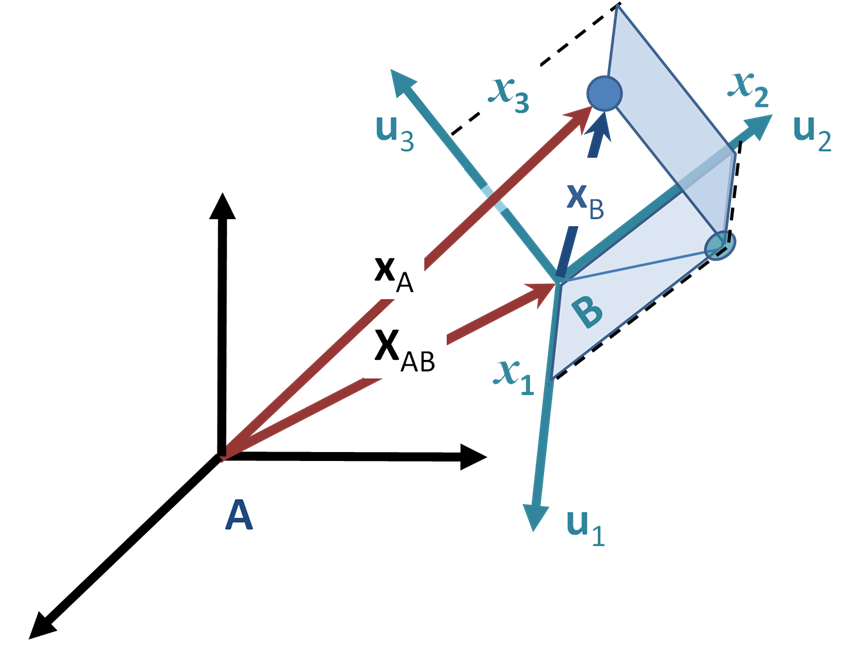
\includegraphics[scale=0.23]{images/moving-coordinate-systems.PNG}
    \caption{
    Visual of two coordinate frames: the inertial frame $A$, and the body frame $B$ from (citation here).
    The point $x$ is observed with vector $x_A$ in the $A$ frame, but the same point $x$ is observed with vector
    $x_B$ in the $B$ frame.
    By aligning several observations in both frames, a spacecraft orientation $x_{AB}$ in the $B$ frame can be
    determined in the $A$ frame.
    } \label{figure:coordinateSystem}
    }
\end{figure}

Once some known object is found by the sensor, these measurements exists in a \textit{body reference frame}.
This reference frame reveals the position of objects with respect to the sensor, but is not fixed to any point.
There exists a separate, fixed frame with which these known objects are recorded to prior to the start of the mission.
This is known as an \textit{inertial reference frame}.
~\autoref{figure:coordinateSystem} depicts the relation between both frames.
Given sensor measurements to a set of points ($X_A, X'_A, X''_A, \ldots$) and inertial frame measurements to the same
objects ($X_B, X'_B, X''_B, \ldots$), the goal of attitude determination involves finding the rotation $X_{AB}$ to
take all points in the sensor frame to the inertial frame (or the inverse).
In short, attitude determination involves taking inertial frame object observations in the body frame, and figuring out
how the spacecraft is oriented in this inertial frame.

From here, the problem becomes aligning vector observations in the body frame with another set of vectors in the
inertial frame.
This is an optimization problem known as \textit{Wahba's problem}.
A popular and simple method to extract an attitude from two vectors in both the inertial and body frame is the
\textit{TRIAD method}.
For all instances where Wahba's problem was present, the TRIAD method was used to extract an orientation.

\subsection{Stellar Based Attitude Determination}\label{subsec:stellarBasedAttitudeDetermination}
Relative to our solar system, the majority of bright stars ($m < 6.0$, or visible from the Earth without a telescope)
\textit{do not visibly move}.
Most of these stars exist hundreds of lightyears away from the solar system.
Observing a tiny change in a star's position from Earth suggests a massive change in position relative to the star.
For many LEO missions, the time it takes for these star positions to change is longer than the length of mission itself.
For longer missions, only then will star dynamics have to be taken into account.
This paper address spacecraft missions where all stars are virtually static in position.

A basic star tracker is composed of a camera, a computer for determining orientation, and a link back to the main
computer.
Once the star tracker on a lost-in-space spacecraft takes a picture, three main pieces of information are known:
\begin{enumerate}
    \item An 2D image of the sky.
    \item Characteristics of the camera hardware (field-of-view, lens structure, \ldots).
    \item All cataloged stars and their 3D positions in the catalog (inertial) frame.
\end{enumerate}

After taking the picture, the pixel positions of potential stars in the image are determined.
This involves finding bright blobs in the image, and computing each blob's center of mass.
To align these stars with the ones in the catalog, the image must be projected into three-dimensional.
This is done using the items in (2) above, and can be a major source of error if these
characteristics are not accurate.
The result of this process are star vectors in the image (body) frame.

By running these image star vectors through a star identification method, a map between the image frame stars and
catalog frame stars is found.
For a given image star $b$ and a catalog star $r$, a map $a$ describes an association ($b, r$) between both stars.
This then reduces to Wahba's problem, and is solved using the TRIAD method to obtain a spacecraft attitude.
	\newcommand{\nsubparagraph}[1]{\subsubsection{#1}}

\section{Related Work}\label{sec:relatedWork}
This section serves to give a brief overview of the different approaches to querying for constellations.
More comprehensive survey papers have been published by Spratling~\cite{spratling:surveyStarIdentification} and
Br\"{a}tt~\cite{bratt:analysisStarIdentification}.

\nsubparagraph{Identification Classes}
The first main class of identification and the focus of this paper is the \textit{subgraph isomorphism} class.
Subgraph isomorphism is NP complete problem which aims to find some 1-to-1 mapping between the vertices (stars) in two
graphs (i.e.\ the database and the image) if it exists~\cite{scott:graphIsomorphismProblem}.
This involves describing and mapping sets of stars between both the database and image in terms of their features
relative to each other.

The second class of identification is the \textit{pattern recognition} class.
In contrast to subgraph isomorphism class, the pattern recognition class commonly deals with larger star sets within
some defined field-of-view and matches patterns rather than features.
Pattern formation typically involves 2D binary matrices (grids), where `1' occupies a cell with a star and `0' occupies
a cell without one~\cite{padgett:gridAlgorithm}.

%
%
%Another notable attempt toward pattern formation utlizes Delaunay Triangulation, as seen from Miri~\cite
%
%Some notable approaches utilize Padgett's~\cite{padgett:gridAlgorithm} and Lee's~\cite{lee:modifiedGridAlgorithm}
%use of binary matrices (grids) to construct patterns, Lindsey~\cite{lindsey:neuralNetworkMethods} and
%Alvelda's~\cite{alvelda:neuralNetworkStar} use of neural networks to optimize pattern similarity, and
%Paladugu's~\cite{paladugu:geneticAlgorithms} use of a genetic algorithm to solve the same pattern similarity problem.

\nsubparagraph{Recursive Property}
Recall that the lost-in-space condition specifies that we do not have any information about the spacecraft's attitude
prior to starting our identification algorithm.
For the majority of a star tracker's lifetime though, this constraint can be relaxed to allow for the use of
\textit{recursive} star identification.
Recursive strategies possess an attitude recorded at time $t$, and perform the identification at a later time $t + dt$.
Two strategies proposed by Samaan (SP-Search and SNA) reduce the amount of candidate stars from the database that could
map to stars from the image~\cite{samaan:recursiveMode}.

\nsubparagraph{Features}
Each star has a position associated with it, be it from a star database or from the image.
Using this position, the most common feature is the interstar angle between two stars, first utilized by Gottlieb to
identify sets of three stars with three angles~\cite{gottlieb:spacecraftAttitudeDetermination}.
Notable strategies with geometric functions utilizing these interstar angles were proposed by:
Groth~\cite{groth:patternMatchingMethod}, Cole \&
Crassidus~\cite{coleAndCrassidis:sphericalTriangleMethod,coleAndCrassidis:planarTriangleMethod}, and
Lang~\cite{lang:astrometryDotNet}.
Another common feature is the interior angle between three stars, where one star exists as a vertex to two other stars.
Liebe uses this in conjunction with interstar angles~\cite{liebe:starTrackersAttitudeDetermination}.

%Each star has a position associated with it, be it from a star catalog or from the image.
%Using this position, the most common feature is the interstar angle between two stars, first utilized by Gottlieb to
%identify sets of three stars with three angles~\cite{gottlieb:spacecraftAttitudeDetermination}.
%Additional geometric functions utilizing these interstar angles were proposed by: Groth (using the log of the sum of
%three interstar angles in a trio~\cite{groth:patternMatchingMethod}), Cole \& Crassidus (treating the angles of a
%star trio as sides to a triangle, and computing the triangle's area and
%torque)~\cite{coleAndCrassidis:sphericalTriangleMethod, coleAndCrassidis:planarTriangleMethod}, and Lang (using the
%differences in interstar angle between a star quad in a localized coordinate system)~\cite{lang:astrometryDotNet}.
%Another common feature is the interior angle between three stars, where one star exists as a vertex to two other stars.
%Liebe uses this in conjuction with interstar angles~\cite{liebe:starTrackersAttitudeDetermination}.

%This feature is used solely by Rousseau (the sine of the closest two closest stars of a trio)
%~\cite{rousseau:starRecognitionAPS}
%and Samaan (the interior angles of three stars)
%~\cite{samaan:nondimensionalStarIdentification},
%and in conjunction with the interstar angles by Liebe~\cite{liebe:starTrackersAttitudeDetermination}.

Each star also has a brightness attached it, a feature less commonly used due to large variance in measurement.
Spratling describes two early strategies to take advantage of this feature.
Scholl proposed the usage of this to remove the need for ambiguity after matching star subsets with angular features
~\cite{scholl:starFieldIdentification}.
Ketchum later introduced the second sequential filtering algorithm, which identifies two stars using their brightness
in comparison to the common trio required of interstar angle strategies~\cite{ketchum:onboardStarIdentification}.
More recent work toward integrating brightness more heavily has been performed by Zhang et
al~\cite{zhang:brightnessReferenced}.

\nsubparagraph{Database Access}
The naive approach to searching for matching features in a subgraph isomorphism approach is to perform a
linear search across the entire database and search for matching subsets.
Early star identification strategies focused on reducing the size of the database to be searched, rather than the search
process itself.
In 1996, Quine (according to Spratling) was the first to reduce the database search time from linear to log time
using a binary search tree~\cite{quine:fastAutonomousStarAcquistion}.
The following year Mortari's "Search-Less Algorithm" was introduced, which utilizes $k$-vectors to search the database
independent of its size~\cite{mortari:kVectorApproach}.

\newcommand{\srightarrow}{\! \rightarrow \!}
\begin{figure}
    \centering{
    % Style for process block.
\tikzstyle{process} = [rectangle, text width=3cm, minimum width=3cm, minimum height=1cm,text centered, draw=black,
fill=orange!30]

% Style for terminal block.
\tikzstyle{terminal} = [rectangle, text width=1.7cm, minimum width=1.7cm, minimum height=1.7cm,text centered,
draw=black, fill=red!30]

% Style for decision block.
\tikzstyle{decision} = [diamond, text width=2cm, minimum width=2.5cm, minimum height=2.5cm,text centered, draw=black,
fill=green!30, inner sep=-10pt]

% Style for line.
\tikzstyle{line} = [draw, -latex']

\begin{tikzpicture}[node distance=1.8cm]
    \node[scale=1](getImage)[terminal]{Get Camera Image};
    \node[scale=1](pickQueryStars) [process, left of=getImage, xshift = -1.7cm] {Pick $k$ Image Stars};
    \node[scale=1](searchCatalog)[process, below of=pickQueryStars] {Search Catalog};
    \node[scale=1](confidentInCatalog)[decision, below of=searchCatalog, yshift=-0.5cm] {$|R| > 0$?};
    \node[scale=1](filterCandidates)[process, below of=confidentInCatalog, yshift=-0.5cm] {Filter Candidates};
    \node[scale=1](confidentAfterFilter)[decision, below of=filterCandidates, yshift=-0.5cm] {Confident in $r$?};
    \node[scale=1](findMap)[process, below of=confidentAfterFilter, yshift=-0.5cm]{Identify};
    \node[scale=1](confidentInMap)[decision, below of=findMap, yshift=-0.5cm] {Confident in $a$?};
    \node[scale=1](returnMap)[terminal, right of=confidentInMap, xshift = 1.7cm] {Return Map};

    \draw[->,>=stealth](getImage) -- node[scale=1.3, yshift=-0.3cm]{$I$}(pickQueryStars);
    \draw[->,>=stealth] (pickQueryStars) -- node[scale=1.3, xshift=0.5cm]{$b$}(searchCatalog);
    \draw[->, >=stealth] (searchCatalog) -- node[scale=1.3, xshift=0.5cm, yshift=-0.15cm]{$R$}(confidentInCatalog);
    \draw[->, >=stealth] (confidentInCatalog) -- node[anchor=east, yshift=0.1cm]{Yes}(filterCandidates);
    \draw[->, >=stealth] (filterCandidates) -- node[scale=1.3, xshift=0.5cm, yshift=-0.15cm]{$r$}(confidentAfterFilter);
    \draw[->, >=stealth] (confidentInMap) -- node[xshift=-0.05cm, yshift=0.2cm]{Yes}(returnMap);
    \draw[->, >=stealth] (confidentAfterFilter) -- node[anchor=east, yshift=0.1cm]{Yes} (findMap);
    \draw[->, >=stealth] (findMap) -- node[scale=1.3, xshift=0.5cm, yshift=-0.15cm]{$a$}(confidentInMap);

    \draw[->, >=stealth] (confidentInCatalog.west) -- ++(-1.1cm, 0cm) node[anchor=south, xshift=0.5cm]{No}
    |- (pickQueryStars.west);
    \draw[->, >=stealth] (confidentAfterFilter.west) -- ++(-1.1cm, 0cm) node[anchor=south, xshift=0.5cm]{No}
    |- (pickQueryStars.west);
    \draw[->, >=stealth](confidentInMap.west) -- ++(-1.1cm, 0cm) node[anchor=south, xshift=0.5cm]{No}
    |- (pickQueryStars.west);
\end{tikzpicture}
    \caption{
    Flowchart depicting the unified identification framework which all strategies here follow.
    Given an image $I$, this process returns a function $h$ whose domain is some subset of the image $b$ and whose
    codomain is a subset of the stellar database, $r$.
    In the event all subsets are exhausted, the function $h: b \srightarrow \emptyset$ is returned (not depicted).
    } \label{figure:unifiedIdentificationFlowchart}
    }
\end{figure}

\nsubparagraph{Mapping}
To identify a star in an image is to pair it with some star in a database.
Gottlieb's strategy used a voting approach to remove the ambiguity after identifying a single star
pair~\cite{gottlieb:spacecraftAttitudeDetermination},
which was later generalized by Kolomenkin to vote for every star in the image~\cite{kolomenkin:geometricVoting}.
The direct match test was proposed by Needleman (according to Tappe), which determines the likelihood of a map based
on how many stars from each frame align with the attitude formed by the map~\cite{needelman:stellarAttitudeAcquisition}.
In an effort to avoid the mapping processes above, Anderson (according to Spratling) proposed the use of storing
permutations of star subsets instead of combinations at the expense of storage~\cite{anderson:autonomousStarSensing}.
The use of neural networks~\cite{lindsey:neuralNetworkMethods,alvelda:neuralNetworkStar} and genetic
algorithms~\cite{paladugu:geneticAlgorithms} have also been proposed to optimize the mapping process.

	\section{Star Identification Methods}\label{sec:starIdentificationMethods}

\subsection{Generic Identification Method}\label{subsec:genericIdentificationMethod}
Each identification method is presented with an image $I$ of all the stars in the image reference frame. The goal of
each method is to find some mapping between the \textit{subset} of the image star vectors $b$ and a subset of the
catalog star vectors $r$. This mapping will be denoted as $a$, for alignment. Complete identification of the all stars
in each image is not the focus.

Every algorithm starts with some combination $c$ from all possible $k$ combinations of $|I|$ stars $C_k^{|I|}$, where
$k = $ the size of the image subset that specific identification method uses. A set of stars from the image $b$ is
selected using the current combination $c$.

Using certain features of $b$, a set of catalog star sets $R$ is obtained. $R$ is a list of catalog star candidates as
to which $b$ could map to. Through some filter process, a single set $r$ from $R$ is then selected. The alignment $a$
is then determined between $r$ and $b$. If all of these steps are successful, then this alignment is returned.
Otherwise, a new combination $c$ is selected and the entire process is repeated. This process is detailed
in~\autoref{figure:genericIdentificationMethodFlowchart}.

\begin{figure}
    \centering{
    % Style for process block.
\tikzstyle{process} = [rectangle, text width=3cm, minimum width=3cm, minimum height=1cm,text centered, draw=black,
fill=orange!30]

% Style for terminal block.
\tikzstyle{terminal} = [rectangle, text width=1.7cm, minimum width=1.7cm, minimum height=1.7cm,text centered,
draw=black, fill=red!30]

% Style for decision block.
\tikzstyle{decision} = [diamond, text width=2cm, minimum width=2.5cm, minimum height=2.5cm,text centered, draw=black,
fill=green!30, inner sep=-10pt]

% Style for line.
\tikzstyle{line} = [draw, -latex']

\begin{tikzpicture}[node distance=1.8cm]
    \node[scale=1](getImage)[terminal]{Get Camera Image};
    \node[scale=1](pickQueryStars) [process, left of=getImage, xshift = -1.7cm] {Pick $k$ Image Stars};
    \node[scale=1](searchCatalog)[process, below of=pickQueryStars] {Search Catalog};
    \node[scale=1](confidentInCatalog)[decision, below of=searchCatalog, yshift=-0.5cm] {$|R| > 0$?};
    \node[scale=1](filterCandidates)[process, below of=confidentInCatalog, yshift=-0.5cm] {Filter Candidates};
    \node[scale=1](confidentAfterFilter)[decision, below of=filterCandidates, yshift=-0.5cm] {Confident in $r$?};
    \node[scale=1](findMap)[process, below of=confidentAfterFilter, yshift=-0.5cm]{Identify};
    \node[scale=1](confidentInMap)[decision, below of=findMap, yshift=-0.5cm] {Confident in $a$?};
    \node[scale=1](returnMap)[terminal, right of=confidentInMap, xshift = 1.7cm] {Return Map};

    \draw[->,>=stealth](getImage) -- node[scale=1.3, yshift=-0.3cm]{$I$}(pickQueryStars);
    \draw[->,>=stealth] (pickQueryStars) -- node[scale=1.3, xshift=0.5cm]{$b$}(searchCatalog);
    \draw[->, >=stealth] (searchCatalog) -- node[scale=1.3, xshift=0.5cm, yshift=-0.15cm]{$R$}(confidentInCatalog);
    \draw[->, >=stealth] (confidentInCatalog) -- node[anchor=east, yshift=0.1cm]{Yes}(filterCandidates);
    \draw[->, >=stealth] (filterCandidates) -- node[scale=1.3, xshift=0.5cm, yshift=-0.15cm]{$r$}(confidentAfterFilter);
    \draw[->, >=stealth] (confidentInMap) -- node[xshift=-0.05cm, yshift=0.2cm]{Yes}(returnMap);
    \draw[->, >=stealth] (confidentAfterFilter) -- node[anchor=east, yshift=0.1cm]{Yes} (findMap);
    \draw[->, >=stealth] (findMap) -- node[scale=1.3, xshift=0.5cm, yshift=-0.15cm]{$a$}(confidentInMap);

    \draw[->, >=stealth] (confidentInCatalog.west) -- ++(-1.1cm, 0cm) node[anchor=south, xshift=0.5cm]{No}
    |- (pickQueryStars.west);
    \draw[->, >=stealth] (confidentAfterFilter.west) -- ++(-1.1cm, 0cm) node[anchor=south, xshift=0.5cm]{No}
    |- (pickQueryStars.west);
    \draw[->, >=stealth](confidentInMap.west) -- ++(-1.1cm, 0cm) node[anchor=south, xshift=0.5cm]{No}
    |- (pickQueryStars.west);
\end{tikzpicture}
    \caption{
    Flowchart depicting a general star identification process.
    Given an image $I$, this processes returns an alignment $a$ mapping some subset of the input $b$ to a subset of
    the catalog $r$.
    } \label{figure:genericIdentificationMethodFlowchart}
    }
\end{figure}

% Leaving this out for now. The flowchart should explain the process better.
%\begin{algorithm}[H]
%    \caption{Generic Star Identification Method} \label{algorithm:genericStarIdentification}
%    \begin{algorithmic}[1]
%        \Procedure{Identify}{}
%        \State $I \gets $ all stars from image
%        \For{$c \in r_k^{|I|}$}
%        \State $b \gets \{I(c_1), I(c_2), I(c_3), \dots, I(r_k)\}$
%        \State $R \gets $ catalog star sets, each set of size $=k$
%        \State $r \gets $ a single set from $R$ that matches $b$
%        \State $a \gets $ an alignment between $b$ and $r$
%        \\
%        \If{the steps above are successful}
%        \State \textbf{return} $a$
%        \EndIf
%        \EndFor
%        \EndProcedure
%    \end{algorithmic}
%\end{algorithm}

% Citation: https://digitalcommons.usu.edu/cgi/viewcontent.cgi?article=2723&context=etd AND Gottlieb.
\subsection{Gottlieb's Angle Method}\label{subsec:gottlieb'sAngleMethod}
In 1978, Gottlieb (citation here) developed the Polygon Angular Matching method. Starting with an image $I$, two stars
$b = (b_1, b_2)$ are selected arbitrarily. The corresponding angular separation between each of these stars from a
defined observer is computed, which is denoted as $\theta^{12}$. All possible pairs $(r_i, r_j)$ in the catalog are then
selected such that condition~\eqref{eq:angleRequirement} holds. The set that holds these pairs is denoted as $R$.

\begin{align}
    \label{eq:angleRequirement}
    \begin{split}
        | \theta(r_i, r_j) - \theta^{12} | < 3 \sigma
    \end{split}
\end{align}
$\sigma$ represents the deviation of the uncertainty between the star sensor measurements and the points defined in the
catalog. Assuming the noise follows a Gaussian distribution, it follows that 99.7\% of all true pairs will be within
this range.

If there exists more than one catalog pair after this reduction, then this process is repeated for
$\theta^{13}, \theta^{14}, \dots,$ and so on until a unique pair is found or all possible pairs in the image
have been exhausted. To determine an alignment, a \textit{direct match test} (DMT) is performed.

\begin{algorithm}
    \caption{Angle Identification Method} \label{algorithm:angleIdentification}
    \begin{algorithmic}[1]
        \Procedure{Identify}{}
        \State $I \gets \text{all stars} \text{ from image}$
        \For{$i \gets 1 \text{\textbf{ to }} |I|$}
        \For{$j \gets i + 1 \text{\textbf{ to }} |I| - 1$}
        \State $b \gets (b_i, b_j)$
        \State $R \gets $ catalog pairs that meet~\eqref{eq:angleRequirement} with $b$
        \\
        \If{$|R| = 1$}
        \State $r \gets $ singular pair inside $R$
        \State $a \gets $ \Call{DMT}{$b, r$}
        \State \textbf{return} $a$
        \EndIf
        \EndFor
        \EndFor
        \EndProcedure
    \end{algorithmic}
\end{algorithm}

Tappe (citation here) specifies this DMT method, which extracts an attitude after running this candidate finding step.
Given an image star pair $(b_i, b_j)$ and a catalog star pair $(r_i, r_j)$, an alignment is proposed:
\begin{equation}
    a_1 = (b_i \rightarrow r_i, b_j \rightarrow r_j)
\end{equation}

Wahba's problem (extracting an attitude given vector observations in two coordinate systems) is then solved using the
TRIAD method. This gives a rotation $q_1$ between the image and catalog frames. This process is repeated for the other
possible alignment to obtain a second rotation $q_2$:
\begin{equation}
    a_2 = (b_i \rightarrow r_j, b_j \rightarrow r_i)
\end{equation}

The most likely attitude is determined by predicting which entries in the catalog represent stars in the image using
$q_1$ and $q_2$. The alignment with the most correctly predicted stars is then returned as the resulting attitude.
The general form for this function (accepting an $B$ and $R$ of arbitrary size) is described
in algorithm~\autoref{algorithm:angleHelper}.

\begin{algorithm}
    \caption{Functions for Angle Method} \label{algorithm:angleHelper}
    \begin{algorithmic}[1]
        \Function{DMT}{$b, r$}
        \State $A \gets $ all possible permutations between $b$ and $r$
        \State $M \gets \emptyset$
        \For {$a \in A$}
        \State $q \gets $ \Call{TRIAD}{$a$}
        \State $M \gets M ||$ (stars correctly predicted with $q$)
        \EndFor
        \\
        \State \textbf{return} alignment $a$ associated with \Call{Max}{$M$}
        \EndFunction
    \end{algorithmic}
\end{algorithm}

\subsection{Liebe's Interior Angle Method}\label{subsec:liebe'sInteriorAngleMethod}
In 1995, Liebe (citation here) developed the Liebe Star ID method. Starting with an image $I$, a central star $b_c$ is
selected arbitrarily. The two closest stars in the image to the central star are selected next, denoted as $b_1$ and
$b_2$. Three features are then computed: the angular separation between $b_1$ and $b_c$, the angular separation between
$b_2$ and $b_c$, and the interior angle between $b_1$ and $b_2$ with $b_c$ at the vertex. These are denoted as
$\theta^1, \theta^2,$ and $\phi$ respectively.

The additional constraint that $\theta^1 < \theta^2$ is imposed before proceeding. If this is not true, then stars
$b_1$ and $b_2$ are swapped and this process is repeated. By adding this restriction to the catalog search, a star
alignment procedure (e.g.\ Tappe's direct match test) is no longer required.

All possible \textit{trios} $R$ in the catalog are then selected such that all of
condition~\eqref{eq:interiorAngleRequirement} hold:
\begin{align}
    \label{eq:interiorAngleRequirement}
    \begin{split}
        |\theta(r_i, r_c) - \theta^1| < 3 \sigma_{\theta}
        \\
        |\theta(r_j, r_c) - \theta^2| < 3 \sigma_{\theta}
        \\
        |\phi(r_i, r_j, r_c) - \phi| < 3 \sigma_{\phi}
        \\
        \theta(r_i, r_c) < \theta(r_j, r_c)
    \end{split}
\end{align}

$\sigma_{\theta}$ and $\sigma_{\phi}$ represent the deviation of measurement-catalog uncertainty of angular separations
and interior angular separations respectively. \textit{Note that the $R$ in this procedure is distinct from the $R$ in
the previous Angle method.}

The star trios in $R$ represent potential catalog maps for the image star trio $(b_1, b_2, b_c)$. Liebe's original
method states that this process should be repeated for all stars in the image, meaning that all stars will be the $b_c$
at one point. By the end, each star in the image will have accrued a set of possible catalog matches $P$. The complete
$B \rightarrow R$ map is found by picking the most frequent catalog star appearing in $P$.

To more closely follow the generic star identification flow, $P$ will not be stored and a only one $b_c$ choice will be
needed to acquire a total match. If a confident match is not found by the first $b_c$ star, then the search process
will be repeated until such a match is found. This entire method is described in
algorithm~\autoref{algorithm:interiorAngleIdentification}.

\begin{algorithm}
    \caption{Interior Angle Identification Method} \label{algorithm:interiorAngleIdentification}
    \begin{algorithmic}[1]
        \Procedure{Identify}{}
        \State $I \gets \text{all stars } \text{ from image}$
        \For{$i \gets 1 \text{\textbf{ to }} |I|$}
        \For{$j \gets i + 1 \text{\textbf{ to }} |I| - 1$}
        \For{$k \gets j + 1 \text{\textbf{ to }} |I| - 2$}
        \State $b \gets (b_i, b_j)$
        \State $R \gets $ catalog trios that meet~\eqref{eq:interiorAngleRequirement} with $b$
        \\
        \If{$|R| = 1$}
        \State $(r_i, r_j) \gets $ singular pair inside $R$
        \State $a \gets (b_i \rightarrow r_i, b_j \rightarrow r_j, b_k \rightarrow r_k)$
        \State \textbf{return} $a$
        \EndIf
        \EndFor
        \EndFor
        \EndFor
        \EndProcedure
    \end{algorithmic}
\end{algorithm}

\subsection{Cole and Crassidus's Spherical Triangle Method}\label{subsec:coleAndCrassidus'sSphericalTriangleMethod}
In 2004, Cole and Crassidus (citation here) developed the Spherical Triangle method. Starting with an image $I$, three
stars $b = b_1, b_2, b_3)$ are selected arbitrarily. Treating the trio as a spherical triangle, the spherical area and
moment are computed. This is denoted as $a^{123}$ and $\imath^{123}$ respectively. Similar to Gottlieb's method, star
\textit{trios} $R$ are selected from the catalog such that the all of condition~\eqref{eq:triangleRequirement} hold:
\begin{align}
    \begin{split}
        \label{eq:triangleRequirement}
        | a(r_i, r_j, r_k) - a^{123} | < 3 \sigma_a
        \\
        | \imath(r_i, r_j, r_k) - \imath^{123} | < 3\sigma_{\imath}
    \end{split}
\end{align}
$\sigma_a$ and $\sigma_{\imath}$ represent the deviation of measurement-catalog uncertainty of spherical areas and
moments respectively.

If there exists more than one catalog trio, then a \textit{pivot} is performed. The pivoting process is repeated until
a unique match in $R_{t=1}$ is found, or all possible iterations of the third image star are exhausted. The entire
catalog search procedure is repeated until a unique catalog trio is found, or all trios in the image have been used.
This procedure is described in algorithm~\autoref{algorithm:triangleIdentification}.

\begin{algorithm}
    \caption{Triangle Method Identification} \label{algorithm:triangleIdentification}
    \begin{algorithmic}[1]
        \Procedure{Identify}{}
        \State $I \gets \text{all stars} \text{ from image}$
        \For{$i \gets 1 \text{\textbf{ to }} |I|$}
        \For{$j \gets i + 1 \text{\textbf{ to }} |I| - 1$}
        \For{$k \gets j + 1\text{\textbf{ to }} |I| - 2$}
        \State $R \gets$ \Call{Pivot}{$b_i, b_j, b_k, \emptyset$}
        \If{$R \neq \emptyset$}
        \State \textbf{return} $R$
        \EndIf
        \EndFor
        \EndFor
        \EndFor
        \EndProcedure
    \end{algorithmic}
\end{algorithm}

The pivot procedure starts by setting $R$ to $R_{t=1}$, beginning the pivot with the trio set that was just queried
for. A second set of trios $R_{t=2}$ is retrieved using $\bar{b} = (b_1, b_2, b_4)$, keeping $b_1$ and $b_2$ constant
but changing the third image star. All star trios in $R_{t=1}$ that do not match a trio in $R_{t=2}$ by
\textit{two stars} (a partial match) are removed from $R_{t=1}$. Note that the \Call{Pivot}{$b_i, b_j, b_k, R_1$} call
inside algorithm~\autoref{algorithm:triangleIdentification} defines $R_1 = \emptyset$, which requires a "check" on
lines 2 and 3 of algorithm~\autoref{algorithm:triangleHelper}.

\begin{algorithm}
    \caption{Functions for Triangle Alignment Determination} \label{algorithm:triangleHelper}
    \begin{algorithmic}[1]
        \Function{PartialMatch}{$R_1, R_t$}
        \If {$R_t = \emptyset$} \Comment $t = 1$, no previous set.
        \State \textbf{return} $R_1$
        \EndIf
        \\
        \State $\bar{R_1} \gets \emptyset$
        \ForAll {$v \in R_t$}
        \ForAll {$u \in R_1$}
        \If{two stars in $v$ exist in $u$}
        \State $\bar{R_1} \gets \bar{R_1} || v$
        \State \textbf{break}
        \EndIf
        \EndFor
        \EndFor
        \State \textbf{return} $\bar{R_1}$
        \EndFunction
        \\
        \Function{Pivot}{$b_i, b_j, b_k, R_1$}
        \State $b \gets (b_j, b_j, b_k)$
        \State $R_t \gets $ catalog trios that meet~\eqref{eq:triangleRequirement} with $b$
        \State $R_1 \gets $ \Call{PartialMatch}{$R_t, R_1$}
        \\
        \If{$|R_1| = 1$}
        \State \textbf{return} $R_1$
        \ElsIf{$|R_1| = 0$}
        \State \textbf{return} $\emptyset$
        \Else
        \State $\hat{b_k} \gets \text{an unused star in this pivot}$
        \State \textbf{return} \Call{Pivot}{$b_i, b_j, \hat{b_k}, R_1$}
        \EndIf
        \EndFunction
    \end{algorithmic}
\end{algorithm}

Cole and Crassidus don't specify alignment determination steps, so Tappe's DMT process is used to complete the star
identification process. Given an image star trio $(b_i, b_j, b_k)$ and a catalog star trio $(r_i, r_j, r_k)$, an
alignment is proposed:
\begin{equation}
    a_1 = (s_i \rightarrow r_i, b_j \rightarrow r_j, b_k \rightarrow r_k)
\end{equation}

The TRIAD method only uses two vector observations from each frame, meaning that the $b_k \rightarrow r_k$ map is
disregarded as the first rotation $q_1$ is computed. This process is repeated for all 5 other possible alignments to
get $q_2, q_3, \dots, q_6$.
\begin{description}
    \item [$a_1 = $] $(s_i \rightarrow r_i, b_j \rightarrow r_j, b_k \rightarrow r_k)$
    \item [$a_2 = $] $(s_i \rightarrow r_i, b_j \rightarrow r_k, b_k \rightarrow r_j)$
    \item [$a_3 = $] $(s_i \rightarrow r_j, b_j \rightarrow r_i, b_k \rightarrow r_k)$
    \item [$a_4 = $] $(s_i \rightarrow r_j, b_j \rightarrow r_k, b_k \rightarrow r_i)$
    \item [$a_5 = $] $(s_i \rightarrow r_k, b_j \rightarrow r_i, b_k \rightarrow r_j)$
    \item [$a_6 = $] $(s_i \rightarrow r_k, b_j \rightarrow r_j, b_k \rightarrow r_i)$
\end{description}

For all six attitudes, the $a$ yielding the most correctly predicted stars is returned as the resulting attitude.

\subsection{Cole and Crassidus's Planar Triangle Method}\label{subsec:coleAndCrassidus'sPlanarTriangleMethod}
In 2006, Cole and Crassidus (citation here) developed the Planar Triangle method. This is identical to their Spherical
Triangle method, with the exception that each image trio $b = (b_i, b_j, b_k)$ is represented as a planar triangle
instead of a spherical one.

Computing the spherical moment requires the use of recursion, which could be costly in slower hardware to obtain more
precision. The Planar Triangle method avoids this by computing the planar area and moment instead, which do not require
this recursive step.

% Mortari introduced the use of \textit{search-less} catalog access using the $k$-vector approach, but this will not be
% discussed in this paper.
\subsection{Mortari's Pyramid Star Identification Method}\label{subsec:mortari'sPyramidStarIdentificationMethod}
In 2004, Mortari (citation here) developed the Pyramid method. Starting with an image $I$, three stars
$b = (b_1, b_2, b_3)$ are selected to avoid the persistence of false stars. This is specified in lines 19 to 23 in
algorithm~\autoref{algorithm:pyramidIdentification}. The corresponding angular separation between each distinct
permutation of the three is computed, denoted as $\theta^{12}, \theta^{13}, \theta^{23}$. All possible
\textit{pair sets} $R^{12}, R^{13}, R^{23}$ are selected from the catalog such that
condition~\eqref{eq:angleRequirement} holds for each respective $\theta$. The common stars between each of these $R$
sets is then determined, yielding $T^1, T^2, $ and $T^3$. If there exists a sole element inside each $T$, then a
secondary verification involving guessing a nearby star is performed. Once this verification step is past, an
alignment is then returned. This entire process is described in algorithm~\autoref{algorithm:pyramidIdentification}.

\begin{algorithm}
    \caption{Pyramid Identification Method} \label{algorithm:pyramidIdentification}
    \begin{algorithmic}[1]
        \Function {FindCatalogStars} {$b, I$}
        \State $R^{ij} \gets$ catalog pairs that meet~\eqref{eq:angleRequirement} with ($b_i, b_j$)
        \State $R^{jk} \gets$ catalog pairs that meet~\eqref{eq:angleRequirement} with ($b_i, b_j$)
        \State $R^{ik} \gets$ catalog pairs that meet~\eqref{eq:angleRequirement} with ($b_i, b_k$)
        \\
        \State $T^i \gets $ \Call{Common}{$R^{ij}, R^{ik}, \emptyset$}
        \State $T^j \gets $ \Call{Common}{$R^{ij}, R^{jk}, T^i$}
        \State $T^k \gets $ \Call{Common}{$R^{ik}, R^{jk}, T^i \cap T^j$}
        \\
        \If{$|T^i| = 1 $ \textbf{and} $|T^j| = 1 $ \textbf{and} $|T^k| = 1$}
        \State $r \gets $ singular stars in $T_i, T_j, T_k$
        \If{\Call{Verify}{$r, b, I$} is \textbf{true}}
        \State \textbf{return} $r$
        \Else
        \State \textbf{return} $\emptyset$
        \EndIf
        \EndIf
        \EndFunction
        \\
        \Procedure{Identify}{}
        \State $I \gets \text{all stars } s \text{ from image}$
        \For{$dj \gets 1 \text{\textbf{ to }} |I| - 2$}
        \For{$dk \gets 1 \text{\textbf{ to }} |I| - 1 - dj$}
        \For{$k \gets i \text{\textbf{ to }} |I| - dj - dk$}
        \State $j \gets i + dj$
        \State $k \gets j + dk$
        \\
        \State $b \gets (b_i, b_j, b_k)$
        \State $r \gets$ \Call{FindCatalogStars}{$b, I$}
        \If{$r \neq \emptyset$}
        \State $a \gets (b_i \rightarrow r_i, b_j \rightarrow r_j, b_k \rightarrow r_k)$
        \State \textbf{return} $a$
        \EndIf
        \EndFor
        \EndFor
        \EndFor
        \EndProcedure
    \end{algorithmic}
\end{algorithm}

To find the common stars between two sets of \textit{pairs} $R^{ab}$ and $R^{ac}$, they must be flattened into a single
dimensional set. These new sets are denoted as $\bar{R}^{ab}$ and $\bar{R}^{ac}$ respectively. The function
\Call{Common}{$R^{ab}, R^{ac}, E$} in algorithm~\autoref{algorithm:pyramidHelpers} also specifies an $E$ parameter,
which acts as a "exclusion" set. Once a common star is found (e.g.\ $T^i$), it follows that the next common star to be
found (e.g.\ $T^j$) should not include this previously found star.

The second verification step is denoted as \Call{Verify}{$r, b, I$} in
algorithm~\autoref{algorithm:pyramidHelpers}. This function starts by selecting a nearby star to $b$ in the image $b_e$.
The angular separation between each star in $b$ is computed, generating $\theta^{ie}, \theta^{je}, \theta^{ke}$.
Again, three sets of catalog pairs $R^{ie}, R^{je}, R^{ke}$ are selected such that
condition~\eqref{eq:angleRequirement} holds for each respective $\theta$. If the common star between all $R$ sets
exists near the given $r$ set, then the test past. Otherwise, the test fails.

\begin{algorithm}
    \caption{Functions for Pyramid Alignment Determination} \label{algorithm:pyramidHelpers}
    \begin{algorithmic}[1]
        \Function{Common}{$R^{ab}, R^{ac}, F$}
        \State $\bar{R}^{ab} \gets $ \Call{Flatten}{$R^{ab}$} \Comment set of pairs (2D) to 1D set
        \State $\bar{R}^{ac} \gets $ \Call{Flatten}{$R^{ac}$}
        \State \textbf{return} $(\bar{R}^{ab} \cap \bar{R}^{ac}) - F$
        \EndFunction
        \\
        \Function{Verify}{$r, b, I$}
        \State $b_e \gets $ star in image $I$ not in $b$
        \State $R^{ie} \gets$ catalog pairs that meet~\eqref{eq:angleRequirement} with $(b_i, b_e)$
        \State $R^{je} \gets$ catalog pairs that meet~\eqref{eq:angleRequirement} with $(b_j, b_e)$
        \State $R^{ke} \gets$ catalog pairs that meet~\eqref{eq:angleRequirement} with $(b_k, b_e)$
        \\
        \State $T^e \gets $ \Call{Common}{$R^{je}, R^{ke} \cup R^{ie}, \emptyset$}
        \If{$|T^e| = 1$}
        \State $r_e \gets $ singular star in $T^e$
        \If{$r_e$ is near $r$ in catalog}
        \State \textbf{return true}
        \Else
        \State \textbf{return false}
        \EndIf
        \Else
        \State \textbf{return false}
        \EndIf
        \EndFunction
    \end{algorithmic}
\end{algorithm}

\subsection{Toloei's Composite Pyramid Method}\label{subsec:toloei'sCompositePyramidMethod}
In 2014, Toloei (citation here) developed the Novel Stars ID method, which retains all of the key aspects of Motari's
Pyramid method but uses the features from Cole and Crassidus's Planar Triangle method for the query and reference steps
instead of angles. Starting with an image $I$, three stars $b = (b_1, b_2, b_3)$ are selected arbitrarily. Treating the
trio as a planar triangle, the planar area and moment are computed. This is denoted as $a^{123}$ and $\imath^{123}$
respectively. Similar to the Planar Triangle method, star \textit{trios} $R$ are selected from the catalog such that
condition~\eqref{eq:triangleRequirement} hold.

Unlike the triangle methods, no pivot is performed. This searching process is repeated until a unique $R$ is found. A
similar verification process to the Pyramid method is then performed for all possible alignments\ldots.

\begin{table*}[ht]
    \centering {
    \caption{
    Overview table of the different identification methods. Each method's image features, reduction process,
    and alignment process is displayed.
    } \label{tab:identificationMethodOverview}
    \begin{tabular}{  m{0.22\linewidth} || m{0.21\linewidth} | m{0.21\linewidth} | m{0.24\linewidth} }
        & \textbf{Image Features} & \textbf{Reduction} & \textbf{Alignment} \\
        \hline \hline
        \textbf{Angle} & $\theta^{ij}$ & Require $|R|=1$ & \Call{DMT}{$b, r$} \\ \hline
        \textbf{Interior Angle} & $\theta^{ij}, \theta^{jc}, \phi$ & Require $|R| = 1$ & Restrict $\theta^{ic},
        \theta^{jc}$ at Query Time \\ \hline
        \textbf{Spherical Triangle} & Spherical $a^{ijk}, \imath^{ijk}$ & \Call{Pivot}{$b_i, b_j, b_k, R_1$} &
        \Call{DMT}{$b, r$} \\ \hline
        \textbf{Planar Triangle} & Planar $a^{ijk}, \imath^{ijk}$ & \Call{Pivot}{$b_i, b_j, b_k, R_1$} &
        \Call{DMT}{$b, r$} \\ \hline
        \textbf{Pyramid} & $\theta^{ij}, \theta^{ik}, \theta^{jk}$ & Require $|R| = 1$ &
        \Call{Common}{$R^{ab}, R^{ac}, F$}, \Call{Verify}{$r, b, I$} \\ \hline
        \textbf{Composite Pyramid} & Planar $a^{ijk}, \imath^{ijk}$ & \ldots & \ldots
    \end{tabular}
    }
\end{table*}
	\newcommand{\nsubparagraph}[1]{\subparagraph{\textbf{#1}}}
\newcommand{\AVG}{\mathit{AVG}}

\section{Evaluation}\label{sec:evaluation}

TODO: Some text about the section here.
% TODO: Some text about the section here.

\subsection{Experimental Setup}\label{subsec:experimentalSetup}

\begin{subequations}
    \nsubparagraph{Star Catalog:}
    The star catalog used for $K$ is the Hipparcos Input Catalogue.
    Entries that do not have a point $\left( \alpha, \delta \right)$ associated with it were not recorded, giving
    117,956 total stars.
    Out of this entire set, only 4,560 are visible from Earth with the naked eye (apparent magnitude $m$ less than 6.0).
    An additional constraint for each catalog $K^2, K^3, K^3'$ that all stars in each pair or trio be within
    $\psi < 20$ degrees of each other was placed to shorten each algorithm's query step running time.
    All sets $K^2, K^3, K^3'$ construct combinations and permutations using the 4,560 elements and this field of view
    constraint.

    Each entry in $K$ has also been updated from MJD 48319 (March 1991) to MJD 58119 (January 2018).
    The conversion to obtain these updated positions is given below:
    \begin{align}
        \alpha_t &= \alpha_\tau + \mu_\alpha (\tau - t) \\
        \delta_t &= \delta_\tau + \mu_\delta (\tau - t)
    \end{align}
    where $\mu_\alpha$ and $\mu_\delta$ represent the proper motion of some star's right ascension and declination in
    radians per year, $\alpha_\tau$ and $\delta_\tau$ represent the right ascension and declination at time
    $\tau$, $\tau$ represents the time the catalog was recorded, and $t$ represents the time we want to update
    our stars to~\cite{ProperMotion}.
    To construct the point $[ x \ y \ z ]$ for $K$,~\autoref{eq:sphereToCartesian} was used with
    each new $\left(\alpha_t, \delta_t \right)$, with $r = 1$, and then normalized.
\end{subequations}

\nsubparagraph{Benchmark Data Generation:}
Before a raw image can used in the star identification algorithms presented above, it must go through three major
processes: blob detection, centroid determination, and a 2D $\rightarrow$ 3D transformation process.
If a blob is not wholly detected, the centroid is not determined correctly, or the transformation process
is not precise enough, error will exist as input to the algorithm prior to starting.
Given that our goal is to only characterize each star identification algorithm itself, the solution implemented here
involves generating artificial images in 3D space.

Prior to generating the benchmark data, three items are specified: a field of view $\psi$, a \textit{true attitude}
$A^{\nicefrac{\iFrame}{\kFrame}}$, and a 3D vector $\vv{r_f}$ in the catalog frame $\kFrame$ that determines
the center of the image.
The next step is to find all nearby bright stars to the $\vv{r_f}$ in the catalog.
This is denoted as $J$:
\begin{equation}
    J = \set{ j \mid j \in K \land \theta\left( j, \vv{r_f} \right) < \frac{psi}{2} }
\end{equation}
To get the $I$ set, each star in $J$ is then rotated by the true attitude $A^{\nicefrac{\iFrame}{\kFrame}}$:
\begin{equation}
    I = \set{ A^{\nicefrac{\iFrame}{\kFrame}} \cdot j \mid j \in J }
\end{equation}
The set $I$, the field of view, and the rotated image center $\vv{b_f} = A^{\nicefrac{\iFrame}{\kFrame}} \cdot \vv{r_f}$
were then presented to each star identification algorithm.

The first type of noise exists as variance between the relative positions of stars represented in the catalog and those
represented in the image.
This may come from misidentifying the centroids in the image, or from out-of-date catalogs.
To introduce Gaussian noise to an image, we linearly interpolate each star toward some random 3D vector on
the unit sphere spherically (\textit{SLERP}) and distribute the magnitude of the movement normally.
To describe our noise independent of this random vector, we divide our distribution by the current angular separation
between both stars.
Given a star $b_i \in I$, Gaussian noise is applied to obtain the distributed vector $b'_i$ [CITE ME]:
\begin{equation}
    b'_i &= \frac{\sin (1 - K)\Omega}{\sin \Omega}b_i + \frac{\sin \left( K \Omega )\right}{\sin \Omega}b^\star_i
\end{equation}
where $b^\star_i$ represents some random vector whose elements are distributed uniformly, $\Omega$ describes the angle
subtended by the arc, and $K$ describes the magnitude of the interpolation:
\begin{equation}
    \begin{aligned}
        b^\star_i &= \left( \sim U(-1, 1), \sim U(-1, 1), \sim U(-1, 1) \right) \\
        \Omega &= \arccos \left ( b^{\star}_i \cdot b_i \right) \\
        K &= \frac{ \sim N\left(0, \sigma^2\right)}{\theta\left( b^{\star}_i, b_i \right)}
    \end{aligned}
\end{equation}
The additional constraint that the resulting star exist near the image center is also applied:
$\theta\left( b'_i, \vv{r_f} \right) < \nicefrac{\psi}{2}$.
If this is not met, then the process is repeated for this star.

The second type of noise exists as falsely identified sources of light, or spikes in the image.
This involves generating $b^\star_i$ in the same manner that was done for the Gaussian noise process, and normalizing
this.
If the constraint that $b^\star_i$ be near the image center is not met, this process is repeated until such a star is
found.
This is repeated for a set number of spikes.

\nsubparagraph{Hardware:}
All trials were performed on an Intel i7-7700 CPU, 3.60GHz with 8 GB RAM\@.
Each algorithm was implemented in C++14, and compiled without optimization (at \texttt{-O0}).
The exact implementation is available at the following link:
\url{https://github.com/glennga/hoku}.

\subsection{1st Filter: Catalog}\label{subsec:1stFilter:Catalog}
\nsubparagraph{Determining Query $\sigma$:} TODO: Some text here % TODO: Finish this part

The results of each grid search are displayed below, and were used for the following experiments.
\begin{alignat*}{3} % TODO: Format this with \num?
    \text{Angle}&: \sigma_\theta &&= 10^{-4} &&{}\\
    \text{Pyramid}&: \sigma_\theta &&= 10^{-4} &&{} \\
    \text{Dot Angle}&: \sigma_{\theta_{c1}} &&= 10^{-2}, \sigma_{\theta_{c2}} &&= 10^{-2}, \sigma_\phi = 10^{-2} \\
    \text{Spherical Triangle}&: \sigma_a &&= 10^{-9}, \sigma_\imath &&= 10^{-9} \\
    \text{Planar Triangle}&: \sigma_a &&= 10^{-9}, \sigma_\imath &&= 10^{-9} \\
    \text{Composite Pyramid}&: \sigma_a &&= 10^{-9}, \sigma_\imath &&= 10^{-9}
\end{alignat*}

\begin{table}
    \centering {
    %\begin{tabular}{m{0.22\columnwidth}|m{0.2\columnwidth}|m{0.2\columnwidth}|m{0.2\columnwidth}} \toprule
%    \textit{Method} & $y'$ & $S$ & $t_{\AVG} \ (\si{ms})$  \\ \hline
%    Angle & \num{2000} & \num{32} & \num{138.00} \\ \hline
%    Dot Angle & \num{2000} & \num{1440} & \num{171.80} \\ \hline
%    Planar \newline Triangle & \num{2000} & \num{1994} & \num{139.05} \\ \hline
%    Composite \newline Pyramid & \num{2000} & \num{1991} & \num{139.46} \\ \hline
%    Spherical \newline Triangle & \num{2000} & \num{1984} & \num{139.60} \\ \hline
%    Pyramid & \num{1980} & \num{1501} & \num{149.69} \\ \bottomrule
%\end{tabular}

\begin{tabular}{m{0.22\columnwidth}|m{0.2\columnwidth}|m{0.2\columnwidth}|m{0.2\columnwidth}}
    \toprule
    \textit{Method} & $P(r_b \in R)$ & $S$ & $t_{\AVG} \ (\si{ms})$  \\ \hline
    Angle & \num{1.0} & \num{32} & \num{138.00} \\ \hline
    Dot Angle & \num{1.0} & \num{1440} & \num{171.80} \\ \hline
    Planar \newline Triangle & \num{1.0} & \num{1994} & \num{139.05} \\ \hline
    Composite \newline Pyramid & \num{1.0} & \num{1991} & \num{139.46} \\ \hline
    Spherical \newline Triangle & \num{1.0} & \num{1984} & \num{139.60} \\ \hline
    Pyramid & \num{0.99} & \num{1501} & \num{149.69} \\ \bottomrule
\end{tabular}
    \caption{
    Depicts all data associated with testing the query step: the probability that the correct catalog set ($r_b$,
    such that the correct bijection can be formed with $b$) exists in $R$ after querying, the number of trials where the
    resulting $R$ meets the $\abs{R} = 1$ criterion ($S$),
    and the average query running time ($t_{\AVG}$) given images with no noise.
    There exist 2000 runs for each identification method.
    } \label{tab:queryExperimentResults}
    }
\end{table}

\subsubsection{Which method has the fastest catalog query step?}
In~\autoref{sec:starIdentificationMethods}, we describe each method's running time in terms of the number of catalog
accesses $n$ and the size of the $K^d$ catalog.
The $K^2$ catalog, used by the Angle and Pyramid methods, is of size $m_2 = 353,700$ elements with the apparent
magnitude and field-of-view constraints.
The $K^3$ catalog, used by the Spherical Triangle, Planar Triangle, and Composite Pyramid methods is of size
$m_3 = 12,520,359$ elements.
The $K^3'$ catalog, used by the Dot Angle method is of size $m_{3'} = 37,561,083$ elements.
Given the size of each catalog, we hypothesize that the Angle method has the fastest query step
(Pyramid method accesses $K^2$ three times in query step) and the Dot Angle has the slowest query step.

In~\autoref{tab:queryExperimentResults}, the average running time to obtain an $R$ set is displayed for each
identification method given an image for 2000 runs.
The slowest method on average is the Dot Angle method, with its $t_{\AVG} = 30.64 \si{ms}$ longer than the average
$t_{\AVG}$ for all other methods ($30.64 \pm 4.30 \si{ms}$).
Given that this method has the largest catalog, more time should be spent searching for the appropriate elements.

%# http://www.socscistatistics.com/pvalues/normaldistribution.aspx
%import numpy as np
%m_1, m_2, s_1, s_2, n_1, n_2 = 137.9965, 139.051, 4.201486373891982, 3.3748183654828003, 2000, 2000
%z_plane = (m_2 - m_1) / np.sqrt( ((s_1 * s_1) / n_1) + ((s_2 * s_2) / n_2) )
We note that the two fastest methods appear to be Angle method and the Planar Triangle method, but their $t_\AVG$ only
vary by 1.05ms.
Given the null hypothesis that the difference between the Planar Triangle method's query step running time and the
Angle method's query step running time is not significant, $z = 8.75, p < 0.0001$ is found with a two-tailed two
sample $Z$ test.
The running times are very likely not equal.
With the data collected here, the Angle method has the fastest query step.

\subsubsection{Which method meets the $\abs{R} = 1$ criterion the most often?}
The $\abs{R} = 1$ criterion is required for all identification methods, and meeting this criteria as often as possible
prevents additional catalog accesses from occurring.
In~\autoref{tab:queryExperimentResults}, the lowest number of instances where the criterion is met $S$ lies with the
Angle method.
Out of 2000 query steps, the Angle method will have had to perform an additional query step at least 1968 more times.
The Pyramid method only has 499 of these additional query instances, which is a factor of 3.94 less.
The most likely reason for this lies with the selection of the $\sigma_\theta$ parameter, and the fact that only one
feature is used to query $K^2$.
If $\sigma_\theta$ was chosen to be smaller, there would have been more instances where the criterion was met- but
this comes at the cost of being less flexible with Gaussian noise.
The methods using $K^3$ and $K^3'$ have the advantage of being able to create utilize more features of the $b$ set and
distinguish it better, compared to only using $\theta(b, r)$ as the sole feature.

%import numpy as np
%p_1, p_2, n_1, n_2 = (1501 / 2000), ((1994 + 1991 + 1984) / 6000), 2000, 6000
%p = (1501 + 1994 + 1991 + 1984) / (2000 + 6000)
%z = (p_2 - p_1) / np.sqrt( p * (1 - p) * ((1/n_1) + (1/n_2)) )
It appears that the all methods using triangular features (Planar Triangle, Composite Pyramid, Spherical Triangle)
meet the criterion the most often (average of $1989.7 \pm 4.2$ runs).
Again, a larger $\sigma_a$ or $\sigma_\imath$ query parameter may lead to a larger $\abs{R}$.
The next method with the most $\abs{R} = 1$ runs that does not use triangular features is the Pyramid method.
Given the null hypothesis that the difference between the number of $\abs{R} = 1$ Pyramid method runs and the
number of $\abs{R} = 1$ runs for methods with triangular features is not significant, $z = 38.0, p < 0.0001$ is
obtained with a two proportion $Z$ test.
With the data collected here, we find that methods with triangular features are very likely to have more instances
where the $\abs{R} = 1$ criterion is met.

\subsubsection{How effective is the Pyramid method query?}
In the Angle, Spherical Triangle, Planar Triangle, and Composite Pyramid methods, catalog queries can be
generalized to the following SQL query:
\begin{align*}
    \texttt{SELECT } &r \\
    \texttt{FROM } &K^d \\
    \texttt{WHERE } &g_1(r) < g_1(b) + 3\sigma_{g1} \texttt{ AND } g_1(r) > g_1(b) - 3\sigma_{g1} \texttt{ AND } \\
    &g_2(r) < g_2(b) + 3\sigma_{g2} \texttt{ AND } g_2(r) > g_2(b) - 3\sigma_{g2} \\
    &\vdots \\
    &g_d(r) < g_d(b) + 3\sigma_{gd} \texttt{ AND } g_d(r) > g_d(b) - 3\sigma_{gd}
\end{align*}
\begin{align*}
    d =& \text{ number of stars used in the query.} \\
    g =& \text{ function used to obtain a feature. } \\
    \sigma =& \text{ deviation of noise. }
\end{align*}
The Dot Angle method requires the $\theta(r_{c1}, r_{c}) < \theta(r_{c2}, r_c)$ constraint before performing the query
above, but the Pyramid method has the most involved query that involves processing outside of SQL\@.
Three of the queries above must be performed to obtain several different $R$ sets, and the common stars must be
found among each $R$ set to create a singular candidate set for trios.

%# http://www.socscistatistics.com/pvalues/normaldistribution.aspx
%import numpy as np
%m_1, m_2, s_1, s_2, n_1, n_2 = 0.99, 1.0, 0.09949874371066202, 0, 2000, 2000
%z = (m_2 - m_1) / np.sqrt( ((s_1 * s_1) / n_1) + ((s_2 * s_2) / n_2) )
There exist several areas where the Pyramid could drop in accuracy here.
In~\autoref{tab:queryExperimentResults}, the frequency of the correct $r$ for some $b$ existing in $R$ is displayed
for each identification method.
The Pyramid method is shown to have a 0.01\% difference from the 100\% accuracy of each other method.
Given the null hypothesis that this difference is not significant, $z= 4.49, p < 0.0001$ is obtained with a one tailed
two sample $Z$ test.
With the data collected here, we find that the Pyramid method's query step is less accurate than other identification
methods.
Although small, this error will propagate to the next steps and will result in more catalog accesses.

\subsection{2nd Filter: Catalog Candidates}\label{subsec:2ndFilter:CatalogCandidates}
\begin{figure}
    \centering{
    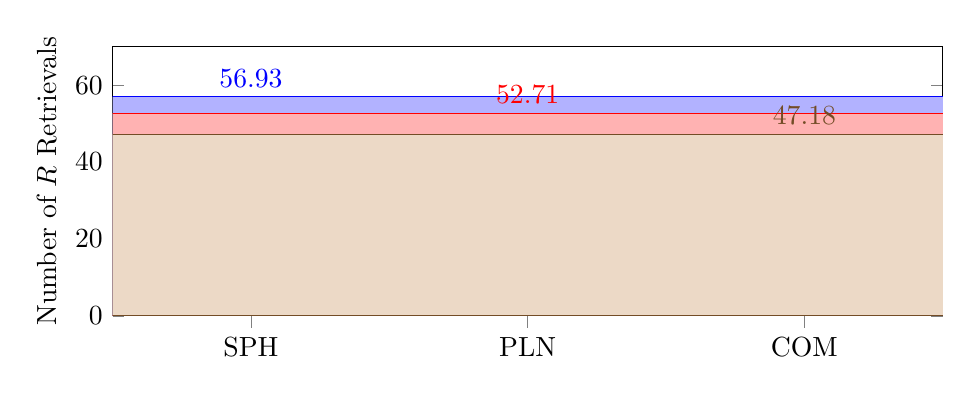
\begin{tikzpicture}
    \begin{axis}[
    ybar,
    width=\linewidth, height=5cm,
    ylabel={Number of $R$ Retrievals}, ylabel near ticks, ymin=0, ymax=70,
    xticklabels={SPH, PLN, COM},
    xtick={1, 2, 3}, xmin=0.5, xmax=3.5, xtick pos=left,
    nodes near coords, nodes near coords align={vertical},
    every axis plot/.append style={
    ybar,
    bar width=40,
    bar shift=0pt,
    fill
    }
    ]
        \addplot coordinates {(1, 56.93)}; % SPH
        \addplot coordinates {(2, 52.71)}; % PLN
        \addplot coordinates {(3, 47.18)};
    \end{axis}
\end{tikzpicture}

%SELECT AVG(QueryCount), IdentificationMethod
%FROM REDUCTION
%WHERE rowid IN (
%    SELECT rowid
%    FROM REDUCTION
%    WHERE (IdentificationMethod LIKE 'Plane' OR IdentificationMethod LIKE 'Sphere')
%    AND ShiftDeviation < 1.0e-3 AND ShiftDeviation > 1.0e-5 AND FalseStars = 0
%    AND QueryCount > 1
%)
%GROUP BY IdentificationMethod

%SELECT AVG(QueryCount)
%FROM REDUCTION
%WHERE rowid IN (
%    SELECT rowid
%    FROM REDUCTION
%    WHERE IdentificationMethod LIKE 'Composite'
%    AND ShiftDeviation < 1.0e-3 AND ShiftDeviation > 1.0e-5 AND FalseStars = 0
%    AND QueryCount > 1
%)
    \caption{
    Depicts the average number of catalog accesses required to obtain a $r$ set for methods with triangular
    features given $\sigma = \ang{0.0001}$ of Gaussian noise.
    To characterize the pivoting method itself, we only display instances where $\abs{R} \neq 1$ with the first $b$
    selection.
    The Spherical Triangle method (SPH) has 1952 / 2000 runs matching the criteria before, the Planar Triangle
    method (PLN) has 1946 runs, and the Composite Pyramid (COM) method has 1957 runs.
    }\label{fig:rPivot}
    }
\end{figure}

\subsubsection{How expensive is the pivoting process?}
%import numpy as np
%m_1, m_2, s_1, s_2, n_1, n_2 = 52.71, 47.18, 56.794658219949106, 47.01765577951369, 1946, 1957
%z = (m_2 - m_1) / np.sqrt( ((s_1 * s_1) / n_1) + ((s_2 * s_2) / n_2) )
As seen previously, identification methods with triangular features have the most number of instances where
$\abs{R} = 1$ given an image with no noise.
In~\autoref{fig:rPivot}, the average number of catalog accesses are displayed for these same methods where the first
$b$ selection does not meet the $R$ criterion given an image with Gaussian noise.
We note that the average number of catalog accesses is higher in methods that use the pivoting processes,
as opposed to those that do not.
Given the null hypothesis that the difference between the Planar Triangle method's number of catalog accesses and
the Composite Pyramid method's number of catalog accesses is not significant, $z = 3.3, p < 0.0001$ is
obtained with a two-tailed two sample $Z$ test.
With the data collected here, we find that the pivoting process results in more catalog accesses on average.
This results in a $6.70\si{ms}$ difference on average between the two.

The pivoting process was only tested with methods using triangular features, whose candidate sets met the $R$ criterion
the most frequently.
An area of interest would be to see the effects of applying this process to methods with angular features (i.e.\ Angle,
Dot Angle, Pyramid).
These methods met the criterion less frequently, and would likely benefit from attempting to reduce the $R$ set before
deciding to choose another $b$ set.

\section{End to End}\label{sec:endToEndEvaluation}

\begin{figure*}
    \centering{
    \begin{subfigure}[b]{0.48\linewidth}
        \begin{tikzpicture}
    \begin{axis}[
    ybar,
    width=\linewidth, height=5cm,
    ylabel={$t \ (\si{ms})$}, ylabel near ticks, ymin=10, ymax=100000,
    xtick={1, 2, 3}, xticklabels={$\ang{0}$, $\ang{0.0001}$, $\ang{0.01}$},
    xlabel={$\sigma$ (degrees)}, xmin=0.5, xmax=3.5, xtick pos=left, point meta=rawy,
    nodes near coords, every node near coord/.append style={rotate=90, anchor=west,
    /pgf/number format/.cd,fixed,precision=6},
    legend style={at={(0.5,-0.35)}, anchor=north,legend columns=-1},
    bar width=7, ymode=log, log origin=infty, max space between ticks=20
    ]
        \addplot coordinates {(1, 1197.43) (2, 1349.07) (3, 6509.00)};
        \addplot coordinates {(1, 160.68) (2, 161.80) (3, 872.22)};
        \addplot coordinates {(1, 323.94) (2, 339.23) (3, 392.29)};
        \addplot coordinates {(1, 324.35) (2, 328.85) (3, 352.24)};
        \addplot coordinates {(1, 170.79) (2, 171.53) (3, 364.04)};
        \addplot coordinates {(1, 405.53) (2, 1545.45) (3, 362.30)};
        \legend{ANG, INT, SPH, PLN, PYR, COM}
    \end{axis}
\end{tikzpicture}
    \end{subfigure}
    \begin{subfigure}[b]{0.48\linewidth}
        \begin{tikzpicture}
    \begin{axis}[
    ybar,
    width=\linewidth, height=5cm,
    ylabel={$a(h, b)$}, ylabel near ticks, ymin=0, ymax=1.3,
    xtick={1, 2, 3}, xticklabels={$\ang{0}$, $\ang{0.0001}$, $\ang{0.01}$},
    xlabel={$\rho$ (degrees)}, xmin=0.5, xmax=3.5, xtick pos=left,
    nodes near coords, every node near coord/.append style={rotate=90, anchor=west},
    legend style={at={(0.5,-0.35)}, anchor=north,legend columns=-1},
    bar width=7
    ]
        \addplot coordinates {(1, 0.977) (2, 0.973) (3, 0.004)};
        \addplot coordinates {(1, 1.0) (2, 1.0) (3, 0.706)};
        \addplot coordinates {(1, 1.0) (2, 0.814) (3, 0.025)};
        \addplot coordinates {(1, 1.0) (2, 0.862) (3, 0.025)};
        \addplot coordinates {(1, 0.999) (2, 0.999) (3, 0)};
        \addplot coordinates {(1, 1.0) (2, 0.003) (3, 0)};
        \legend{ANG, INT, SPH, PLN, PYR, COM}
    \end{axis}
\end{tikzpicture}
    \end{subfigure}
    \caption{
    Both plots represent some statistic about the resulting bijection $f$ produced by each identification method
    given some image with varying Gaussian noise.
    The left plot depicts the average time to obtain $f$, and the right plot depicts the average accuracy of $f$.
    There exist 2000 runs for each identification method, with a 500 $b$ selection bound.
    }\label{fig:gaussianNoise}
    }
\end{figure*}

\begin{figure*}
    \centering{
    \begin{subfigure}[b]{0.48\linewidth}
        \begin{tikzpicture}
    \begin{axis}[
    ybar,
    width=\linewidth, height=5cm,
    ylabel={$t \ (\si{ms})$}, ylabel near ticks, ymin=10, ymax=100000,
    xtick={1, 2, 3}, xticklabels={0, 6, 12},
    xlabel={$\omega$}, xmin=0.5, xmax=3.5, xtick pos=left, point meta=rawy,
    nodes near coords, every node near coord/.append style={rotate=90, anchor=west,
    /pgf/number format/.cd,fixed,precision=2},
    legend style={at={(0.5,-0.35)}, anchor=north,legend columns=-1},
    bar width=7, ymode=log, log origin=infty, max space between ticks=20
    ]
        \addplot coordinates {(1, 1197.43) (2, 1737.94) (3, 2431.58)};
        \addplot coordinates {(1, 160.68) (2, 209.36) (3, 280.54)};
        \addplot coordinates {(1, 323.94) (2, 355.54) (3, 386.20)};
        \addplot coordinates {(1, 324.35) (2, 350.60) (3, 390.41)};
        \addplot coordinates {(1, 170.79) (2, 183.71) (3, 195.53)};
        \addplot coordinates {(1, 405.53) (2, 685.07) (3, 972.04)};
        \legend{ANG, DOT, SPH, PLN, PYR, COM}
    \end{axis}
\end{tikzpicture}
    \end{subfigure}
    \begin{subfigure}[b]{0.48\linewidth}
        \begin{tikzpicture}
    \begin{axis}[
    ybar,
    width=\linewidth, height=5cm,
    ylabel={Accuracy of Map, \texttt{ACC}}, ylabel near ticks, ymin=0, ymax=1.4,
    xtick={1, 2, 3}, xticklabels={0, 6, 12},
    xlabel={$\omega$}, xmin=0.5, xmax=3.5, xtick pos=left,
    nodes near coords, every node near coord/.append style={rotate=90, anchor=west,
    /pgf/number format/.cd,fixed,precision=4},
    legend style={at={(0.5,-0.35)}, anchor=north,legend columns=-1},
    bar width=7
    ]
        \addplot coordinates {(1, 0.977) (2, 0.979) (3, 0.960)};
        \addplot coordinates {(1, 1.0) (2, 0.982) (3, 0.965)};
        \addplot coordinates {(1, 1.0) (2, 0.840) (3, 0.696)};
        \addplot coordinates {(1, 1.0) (2, 0.845) (3, 0.703)};
        \addplot coordinates {(1, 0.999) (2, 0.999) (3, 0.995)};
        \addplot coordinates {(1, 1.0) (2, 0.994) (3, 0.973)};
        \legend{ANG, INT, SPH, PLN, PYR, COM}
    \end{axis}
\end{tikzpicture}
    \end{subfigure}
    \caption{
    Both plots represent some statistic about the resulting bijection $f$ produced by each identification method
    given some image with varying amounts of spikes (false stars).
    The left plot depicts the average time to obtain $f$, and the right plot depicts the average accuracy of $f$.
    There exist 2000 runs for each identification method, with a 500 $b$ selection bound.
    }\label{fig:falseNoise}
    }
\end{figure*}

\subsubsection{Which method is the most accurate under Gaussian noise?}

\subsubsection{Which method is the fastest under Gaussian noise?}

\subsubsection{Which method is the most accurate under false star noise?}

\subsubsection{Which method is the fastest under false star noise?}
	\section{Conclusion}\label{sec:conclusion}
Attitude determination is a vital part of all spacecraft missions.
Previously, devices such as magnetometers and Sun sensors would give one observation each in both the body and inertial
frames.
The advantage of star trackers is the presentation of multiple observations with just one device.
Star identification is the process associated that maps observations found in the body frame (i.e.\ the image) to the
inertial frame (i.e.\ the catalog).

Gottlieb's Angle method, Liebe's Dot Angle method, Motari's Pyramid method, Cole and Crassidis's Spherical and
Planar Triangle method, and Toloei's Composite Pyramid method were adjusted to fit a general identification flow
and were analyzed in terms of their query, reduction, and identification steps.
Portions that were interchangeable amongst all methods such as database access and centroid determination were
normalized or removed to focus on the star identification aspect itself.

In all experiments, the Pyramid method ranked first (or close to first) in running time and fairly high in accuracy.
The average short running time is a result of a relatively fast query step, and its accuracy can be attributed to the
verification procedure at identification time.
The Pyramid method is the least sensitive to hyperparameter changes in terms of query size response and accuracy
response.
This method produced the lowest number of catalog candidate sets for a given query, and is the most tolerant of
both Gaussian noise and false stars.

The Angle method had the fastest query step, which stems from the small catalog ($\sim$35 times smaller than
the next larger catalogs, the triangle catalogs).
There were a few instances where the accuracy of the Angle method was greater than the Pyramid method, but this came
at the cost of runtime.
The results produced by the query step heavily impacted the reduction and identification runtime.
For the no noise end-to-end case, this method was a factor of MP200 times slower than the next slowest method (Dot
Angle method).

The Dot Angle method is the most sensitive to hyperparameter changes, but had a larger ideal region than the other
methods.
The catalog for this method was $\sim$105 times larger than the Angle method, and consequently had the longest query
step.
This method handles Gaussian noise the best of all other methods, being the second fastest to identify an image and
being first in how accurate the result is.
In terms of false stars, this method ranks last in accuracy.

The accuracy of the Spherical and Planar Triangle methods rank in between for both Gaussian noise and false stars.
The differences between the spherical and planar triangle features are minuscule compared to the algorithms
encapsulating the features themselves.
These methods produced the smallest amount of candidates on average, which was useful in mitigating the highest
theoretical upper bound for catalog accesses.
Unfortunately, these methods were not the fastest nor were they the most accurate.

The Composite Pyramid method, a composite of the Planar Triangle method's features and the Pyramid method's processes,
ranks last in accuracy and average runtime for images with Gaussian noise 2nd in accuracy for images with just
false stars.
Combining the two methods also means combining the filters associated with each, and the results show inconsistent
runtime due to failing at different stages of the algorithm.
Instead of getting the best of both worlds here, the Composite Pyramid method inherits the worst portions of the two.

Overall, the Pyramid method handles both Gaussian noise and false stars the best in a reasonable amount of time.
If one is working with a small field-of-view with limited stars to choose from and Gaussian noise, the Dot Angle
method works best for using one less star than the Pyramid method.
If speed is not a factor but the field-of-view problem still persists, the Angle method should suffice.
    %\section{Acknowledgements}\label{sec:acknowledgements}
\begin{acks}
	We would like to thank Dr. Miguel Nunes, Eric Pilger, and Yosef Ben Gershom from the Hawaii Space Flight Laboratory for providing input toward the creation of software for a first generation star tracker.
\end{acks}
    \balance

%	\nocite{*}
	\bibliographystyle{abbrv}
	\bibliography{include/references}

\end{document}
